\documentclass[pdftex,letterpaper,11pt]{article}%
\usepackage[export]{adjustbox}
\usepackage{multirow}
\usepackage[arabicsections]{dpugatex}
%\usepackage{dpppl}
%\usepackage{lscape}
\usepackage{pdflscape}
\usepackage{longtable}

\usepackage{tikz}

\usepackage[british]{babel}
\usepackage{amssymb,amsmath,warpcol,url,ctable,multirow,caption,threeparttable,float,soul,gensymb}
%\usepackage[noend]{algpseudocode}
\makeatletter
\def\BState{\State\hskip-\ALG@thistlm}
\makeatother


\usepackage{subcaption}


\usepackage{xcolor,colortbl}%Per colorejar cel·les de les taules
\definecolor{verylightgray}{gray}{0.90}
\newcommand{\verylightgray}[1]{\cellcolor{verylightgray}#1}


\usepackage{arydshln} %Per dashed lines
\setlength\dashlinedash{1.5pt}
\setlength\dashlinegap{2.5pt}
\setlength\arrayrulewidth{0.8pt}

\usepackage[utf8]{inputenc}
\usepackage{eurosym}
\usepackage{soul}
\setstcolor{red} % Tatxat vermell pel text a eliminar!!!!
\definecolor{lightgreen}{rgb}{0.564706,0.933333,0.564706}
\newcommand{\miquel}[1]{{\sethlcolor{lightgreen} \hl{#1}} } % To highlight with light green Miquel's comments.
\soulregister\citet7 % These \soulregister commands allow us to avoid problems between soul functions (\hl, \st, ...) and these other functions (\citet,\citep,\ref,\footnote, ...). Include more if it is necessary.
\soulregister\citep7
\soulregister\cite7
\soulregister\ref7
\soulregister\footnote7
\soulregister\textit7
\soulregister\textbf7
\soulregister\textsc7
\soulregister\`7 % for open accents.
\soulregister\'7 % for closed accents.
\soulregister\% 7 % for \%age symbol
\usepackage{tabularx,tabulary}
\usepackage[osf]{mathpazo} % Amb aquest paquet faig ús de la lletra Palatino, la que fan servir Puga, Duranton et al. Amb l'opció [osf] la numeració és "old fashion", però és incompatible amb un títol en negreta i small caps (desapareixen les small caps!). Per tant, per ara opto per NO aplicar aquesta opció.
\usepackage[abs]{overpic}

\usepackage{hyperref}
\definecolor{darkblue}{rgb}{0.0,0.0,0.3}
\hypersetup{colorlinks=true, breaklinks=true, citecolor= darkblue, linkcolor=blue, urlcolor=blue}

\usepackage{chngcntr}

\newcommand{\mc}[3]{\multicolumn{#1}{#2}{#3}}
\newcommand{\mcc}[1]{\multicolumn{1}{c}{#1}}
\newcommand{\mcb}[1]{\multicolumn{1}{c}{\bf #1}}

\newcommand{\mr}[3]{\multirow{#1}{#2}{#3}} % Per fer Files múltiples (seguint el punt de vista de les columnes múltiples.
\newcommand{\mg}[3]{\multicolumn{#1}{#2}{\verylightgray #3}} %Combino el color de les cel·les amb al command de les columnes múltiples.



%\hypersetup{%
 % pdftitle={Race and neighborhoods in the 21$^{\text{st}}$ century},%
 % pdfauthor={Jorge De la Roca (NYU) , Ingrid Gould Ellen (NYU) and Katherine O'Regan (NYU)},%
 % pdfkeywords={race segregation, discrimination}}
%\pdfOpenFitWidth
%\pdfShowBookmarks

\onehalfspacing%
%\doublespacing%

\newenvironment{tablenote}[1]{\begin{list}{}{\vskip-5mm\relax
\setlength{\leftmargin}{#1} \setlength{\rightmargin}{\leftmargin}}
\item[]\footnotesize\vskip-7pt
{\em Notes}:\space\ignorespaces}{\end{list}}

\newcommand{\jdlradded}[1]{#1}
\newcommand{\dpadded}[1]{#1}
\newcommand{\jdlrdeleted}[1]{}
\newcommand{\dpdeleted}[1]{}
\newcommand{\jdlrcomment}[1]{}
\newcommand{\dpcomment}[1]{}
\newcommand{\comment}[1]{}
\newcommand{\martin}[1]{{\color{blue} Martin: [{#1}]}}
\newcommand{\dani}[1]{{\color{purple} Ana: [{#1}]}}

\begin{document}
\begin{titlepage}
\vspace*{1ex}
\begin{minipage}{\textwidth}
\begin{center}%

    {\textsb{\LARGE Bananas and tangerines\\ \textit{Spilled on streets}}}\\[4ex]%

July 2022\vspace{1.5ex}
%
\end{center}
%
\begin{abstract}
    A banana is an elongated, edible fruit, botanically a berry, produced by
    several kinds of large herbaceous flowering plants in the genus Musa. In some
    countries, bananas used for cooking may be called "plantains", distinguishing them
    from dessert bananas. The fruit is variable in size, color, and firmness, but is
    usually elongated and curved, with soft flesh rich in starch covered with a rind,
    which may be green, yellow, red, purple, or brown when ripe. The fruits grow upward
    in clusters near the top of the plant. Almost all modern edible seedless
    (parthenocarp) bananas come from two wild species: Musa acuminata and Musa
    balbisiana. The scientific names of most cultivated bananas are Musa acuminata, Musa
    balbisiana, and Musa x paradisiaca for the hybrid Musa acuminata x M. balbisiana,
    depending on their genomic constitution. The old scientific name for this hybrid,
    Musa sapientum, is no longer used.
\end{abstract}
%
\vspace{1.5ex}
%
Key words: \hskip.25em Bananas, Street network\\
%
\vspace*{-1.5ex}
%
\end{minipage}
\end{titlepage}


% the sections may change, but putting in these as placeholder
\section{Introduction}
\label{sec:intro}

\subsection{why do we care?}

1 paragraph general motivation - framework of urban data science. why everyone would benefit from having this issue solved. cite arcaute on 'recent advances, lobo on 'urban science'. also: alessandretti 2020, louail 2015, barthelemy books (morphogenesis 2018; spatial networks 2022)

2-3 sentences morphometrics (fleischmann, porta, dibble, etc.) diet 2018 on planar map classification. sharifi on urban forms.

1 paragraph problem description - cite cardillo, geisberger, morer (computational costs), maybe venerandi 2016?; vanegas paper on actually *simulating* these spaces

1 paragraph examples - other authors complaining about the issue, without having solved it yet (e.g. best paper ever \citep{vybornova2022automated}); grippa 2018; peponis 2007 merges these into urban blocks (replacing by center lines)

1 paragraph summary of what happens in this paper - 'towards an automated detection of bananas';
method inspired by louf and barthelemy;
tried out on X cities across the world,
from different morphological classes (cite fleischmann);
2 sentences about using OSM as data source, and OSMnx/geopandas/momepy (...) for processing;
code is open source (?) ;

Adding some text here.

\section{Method}
\label{sec:method}

Make a strong case for the fact that our method is very simple (it is not a machine learning algorithm); computationally cheap; AND manages to capture BOTH elongated bananas and intersection bananas with ONE stroke and ONE index, which is possible thanks to the CHARACTERISTIC PATTERNS in urban street networks. As demonstrated in the scatter plot \ref{fig:banana-scatter}...

\begin{figure}
    \centering
    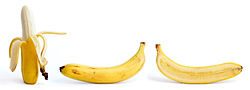
\includegraphics{figures/banana}
    \caption{[Show shape index v. area plot for different continents (?) or for different FUA(s) to show the banana shape in the distribution]}
    \label{fig:banana-scatter}
\end{figure}

% COMMENTING OUT THE NOTES
% - select sample of urban areas (FUA)
% - fetch the data from OSM
% - polygonize the network
% - measure shape charactersitics
%     - TODO: measure initally more than Reock (get a sample from ESDA)
%     - there is a conceptual backbone to this - we know that the artifacts are either
%     small (small intersections) polygons or can be large but then they are very narrow
%     (in between dual carriegaway)
%     - we need a shape metric that captures this relationship
% - identify optimal measurements
%     - plots that help us visually detect a cluster of artifacts
% - derivation of 1-dimensional index
%     - from Roeck and area we can derive one value from which distribution we can
%     identify a cut-off value for artifact/non-artifact polygons
% - cut-off value detection
% - exploration of geographical variation
%     - differences between cities and continents
% - open tools, open data, open code with full reproducibility

\subsection*{Method section on using shape indeces}
mention Sanzana \cite{sanzana_decomposition_2018}, Louf \cite{louf_typology_2014}, ... etc.


\textit{Sanzana et al. propose an algorithm for identification and elimination of ``bad-shaped polygons'', incl. streets/roads/footpaths. Explain that while we have a comparable approach, we are concerned with *cities* while they are concerned with *hydrological models*; and since cities express some certain regularities we can make use of that}

\subsection*{Method section on finding the minimum and using it as a threshold (put part of this in results maybe?)}

\begin{figure}
    \centering
    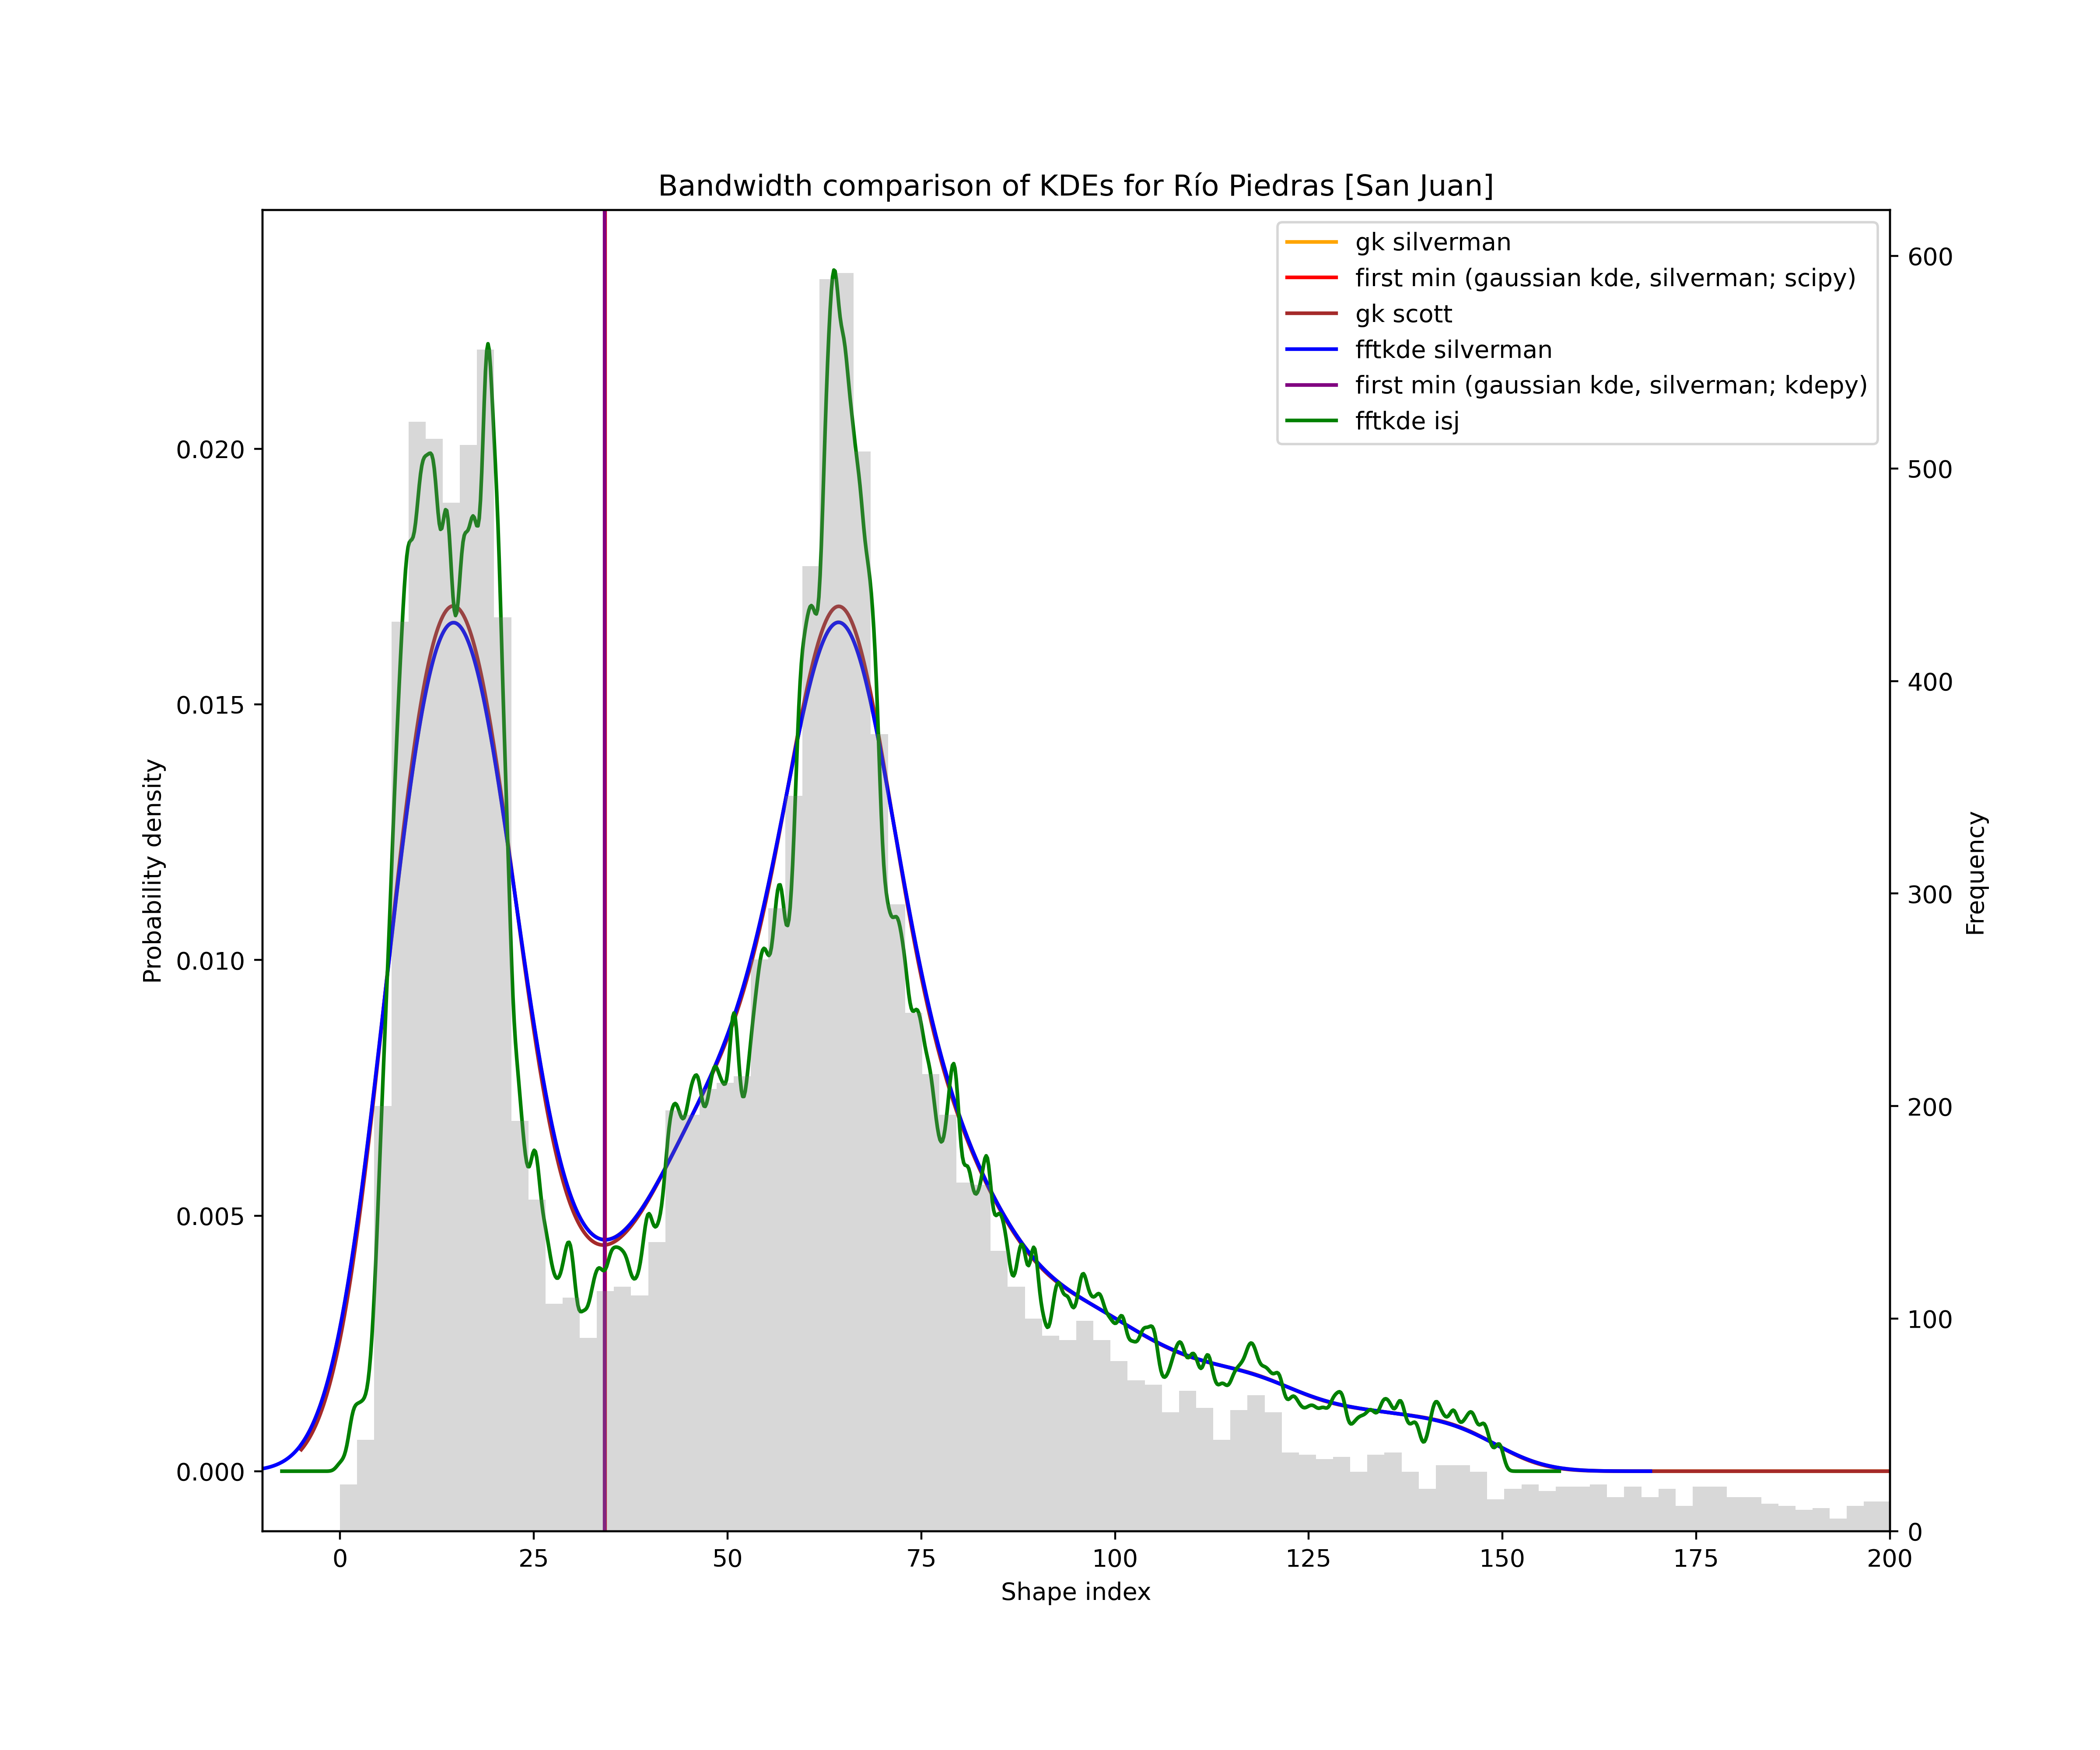
\includegraphics[width=0.5\linewidth]{figures/308}
    \caption{[Above: just a placeholder. Insert here: shape index frequency distribution(s) for FUA X. - show the two-peak pattern]}
    \label{fig:si-dist}
\end{figure}

Many, though not all, shape index frequency distributions for the analyzed FUAs reveal a common feature of two prominent peaks (see Figure \ref{fig:si-dist}). Through visual analysis, we find that these peaks represent two different types of polygons. Most of the polygons from the first (leftmost) peak can be attributed to ``bananas’’ in the street network, whereas most of the polygons from the second (rightmost) peak represent true urban blocks. Therefore, for FUAs that show a pronounced two-peak pattern in their shape index frequency distribution, the minimum \textit{between} the two peaks can be used as shape index threshold: polygons with a shape index below the threshold will most likely be ``bananas’’; polygons with a shape index above the threshold will most likely be true urban blocks. To derive the minimum, we approximate the shape index frequency distribution with a Gaussian kernel density estimation. For bandwidth selection, we use the parametric Silverman method \cite{silverman_using_1981} and find that it gives satisfactory results; non-parametric bandwidth selection methods might be a subject for future work (see section \ref{sec:discussion}). 

Next, comparing the positions of peak 1, peak 2, and shape index threshold for different FUAs with pronounced two-peak patterns, we find that maxima positions vary to a considerably greater extent than minima positions. In other words, shape index thresholds for ``banana’’ identification from morphologically different FUAs lie within a relatively narrow range. We therefore hypothesize that applying a shape index threshold within the range identified from FUAs whose polygons follow a two-peak distribution will allow the identification of ``bananas’’ polygons even for those FUAs whose distributions do not show a two-peak pattern. Applying the … [TBD: lower boundary/median/average/higher boundary] of the empirically derived shape index threshold range to the rest of FUAs indeed reveals ``bananas´´ polygons in all/most FUAs (see Figure \ref{fig:city}).

\section{Results}
\label{sec:results}

- area vs shape plots
    - use all cases together and show multiple shape indices
- Reock as an optimal index (?) [I think it will be the optimal one but we need to verify that]
- 1-dimensional index formula (if we use Reock it is the one from the banana notebook)
- shape-index plots with cut-off values
- plots based on geographical location
    - distributions, Reock-area scatters
    - describe the differences
- formalise the detection workflow


\section{Discussion}
\label{sec:discussion}

How could this be used?

how to move forward? (sneak preview of google summer of code) - the simplification problem can be seen as a problem of the elimination of banana

incorporate further data (ideas: directionality; street names; angles; land use; ...)
use network formalism: on dual approach (intersections = edges): jiang 2004, yang 2022,
rosvall/sneppen; barthelemy paper on shortest path shape

end with a call to action \& 'towards open urban data science'

\bigskip

include in future work:
\begin{itemize}
    \item analyze other regularities in distribution
    \item !! once banana has been found: how to replace it?
    \item non-parametric bandwidth selection
\end{itemize}

\clearpage


\bibliographystyle{apalike}
\bibliography{refs}

\clearpage

\end{document}
